% Arquivo LaTeX template de disserta��o/tese a ser apresentados � CPG do IME-USP
% 
% Vers�o 5: Sex Mar  9 18:05:40 BRT 2012
%
% Cria��o: Jes�s P. Mena-Chalco
% Revis�o: Fabio Kon e Paulo Feofiloff
% Modificado por Rodrigo Campiolo
%  
% Obs: Leia previamente o texto do arquivo README.txt

\documentclass[openany,11pt,twoside,a4paper]{book}

\newcommand{\titulotrabalho} {
    Uma abordagem colaborativa e distribu�da para a detec��o antecipada de incidentes de seguran�a
}

\newcommand{\titulotrabalhoingles} {
    Title
}

\newcommand{\autor} {Rodrigo Campiolo}
\newcommand{\citacaoautor} {CAMPIOLO, R.}
\newcommand{\emailautor} {rcampiolo@utfpr.edu.br}

% Definir macros para o nome da Institui��o, da Faculdade, etc.
\newcommand{\tipotrabalho}{Tese}   %ou Disserta��o ou Qualifica��o
\newcommand{\universidade}{Universidade de S�o Paulo}
\newcommand{\programa}{P�s-Gradua��o em Ci�ncia da Computa��o}
\newcommand{\faculdade}{Faculdade de Ci�ncia da Computa��o}
\newcommand{\instituto}{Instituto de Matem�tica e Estat�stica}
\newcommand{\titulacao}{Doutor} % ou Mestre
\newcommand{\tipoprograma}{Doutorado} % ou Mestrado
\newcommand{\proforientador}{Prof. Dr. Daniel Mac�do Batista}
\newcommand{\profcoorientador}{Prof. Dr. Coorientador}
\newcommand{\profbancaa}{Prof. Dr. NONAME}
\newcommand{\profbancab}{Prof. Dr. NONAME}
\newcommand{\profbancac}{Prof. Dr. NONAME}
\newcommand{\profbancaafac}{IME-USP} 
\newcommand{\profbancabfac}{IME-USP} 
\newcommand{\profbancacfac}{IME-USP} 
\newcommand{\auxiliofinanceiro}{CAPES/CNPq/FAPESP}

\newcommand{\mes}{fevereiro}
\newcommand{\ano}{2014}
\newcommand{\paginas}{x}
% Arquivo LaTeX de exemplo de disserta��o/tese a ser apresentados � CPG do IME-USP
% 
% Vers�o 5: Sex Mar  9 18:05:40 BRT 2012
%
% Cria��o: Jes�s P. Mena-Chalco
% Revis�o: Fabio Kon e Paulo Feofiloff
% Modificado por Rodrigo Campiolo
%  
% Obs: Leia previamente o texto do arquivo README.txt

% ---------------------------------------------------------------------------- %
% Pacotes 
\usepackage[T1]{fontenc}
\usepackage[brazil]{babel}
\usepackage[latin1]{inputenc}
\usepackage[pdftex]{graphicx}           % usamos arquivos pdf/png como figuras
\usepackage{setspace}                   % espa�amento flex�vel
\usepackage{indentfirst}                % indenta��o do primeiro par�grafo
\usepackage{makeidx}                    % �ndice remissivo
\usepackage[nottoc]{tocbibind}  	% acrescentamos a bibliografia/indice/conteudo no Table of Contents
\usepackage{courier}                    % usa o Adobe Courier no lugar de Computer Modern Typewriter
\usepackage{type1cm}            	% fontes realmente escal�veis
\usepackage{listings}                   % para formatar c�digo-fonte (ex. em Java)
\usepackage{titletoc}
%\usepackage[bf,small,compact]{titlesec} % cabe�alhos dos t�tulos: menores e compactos
\usepackage[fixlanguage]{babelbib}
\usepackage[font=small,format=plain,labelfont=bf,up,textfont=it,up]{caption}
\usepackage[usenames,svgnames,dvipsnames]{xcolor}
\usepackage[a4paper,top=2.54cm,bottom=2.0cm,left=2.0cm,right=2.54cm]{geometry} % margens
%\usepackage[pdftex,plainpages=false,pdfpagelabels,pagebackref,colorlinks=true,citecolor=black,linkcolor=black,urlcolor=black,filecolor=black,bookmarksopen=true]{hyperref} % links em preto
\usepackage[pdftex,plainpages=false,pdfpagelabels,pagebackref,colorlinks=true,citecolor=DarkGreen,linkcolor=NavyBlue,urlcolor=DarkRed,filecolor=green,bookmarksopen=true]{hyperref} % links coloridos
\usepackage[all]{hypcap}                    % soluciona o problema com o hyperref e capitulos
\usepackage[round,sort,nonamebreak]{natbib} % cita��o bibliogr�fica textual(plainnat-ime.bst)
\bibpunct{(}{)}{;}{a}{\hspace{-0.7ex},}{,} % estilo de cita��o. Veja alguns exemplos em http://merkel.zoneo.net/Latex/natbib.php

\fontsize{60}{62}\usefont{OT1}{cmr}{m}{n}{\selectfont}

% ---------------------------------------------------------------------------- %
% Cabe�alhos similares ao TAOCP de Donald E. Knuth
\usepackage{fancyhdr}
\pagestyle{fancy}
\fancyhf{}
\renewcommand{\chaptermark}[1]{\markboth{\MakeUppercase{#1}}{}}
\renewcommand{\sectionmark}[1]{\markright{\MakeUppercase{#1}}{}}
\renewcommand{\headrulewidth}{0pt}

% ---------------------------------------------------------------------------- %
\graphicspath{{./figuras/}}             % caminho das figuras (recomend�vel)
\frenchspacing                          % arruma o espa�o: id est (i.e.) e exempli gratia (e.g.) 
\urlstyle{same}                         % URL com o mesmo estilo do texto e n�o mono-spaced
\makeindex                              % para o �ndice remissivo
\raggedbottom                           % para n�o permitir espa�os extra no texto
\fontsize{60}{62}\usefont{OT1}{cmr}{m}{n}{\selectfont}
\cleardoublepage
\normalsize

% ---------------------------------------------------------------------------- %
% Op��es de listing usados para o c�digo fonte
% Ref: http://en.wikibooks.org/wiki/LaTeX/Packages/Listings
\lstset{ %
language=Java,                  % choose the language of the code
basicstyle=\footnotesize,       % the size of the fonts that are used for the code
numbers=left,                   % where to put the line-numbers
numberstyle=\footnotesize,      % the size of the fonts that are used for the line-numbers
stepnumber=1,                   % the step between two line-numbers. If it's 1 each line will be numbered
numbersep=5pt,                  % how far the line-numbers are from the code
showspaces=false,               % show spaces adding particular underscores
showstringspaces=false,         % underline spaces within strings
showtabs=false,                 % show tabs within strings adding particular underscores
frame=single,	                % adds a frame around the code
framerule=0.6pt,
tabsize=2,	                % sets default tabsize to 2 spaces
captionpos=b,                   % sets the caption-position to bottom
breaklines=true,                % sets automatic line breaking
breakatwhitespace=false,        % sets if automatic breaks should only happen at whitespace
escapeinside={\%*}{*)},         % if you want to add a comment within your code
backgroundcolor=\color[rgb]{1.0,1.0,1.0}, % choose the background color.
rulecolor=\color[rgb]{0.8,0.8,0.8},
extendedchars=true,
xleftmargin=10pt,
xrightmargin=10pt,
framexleftmargin=10pt,
framexrightmargin=10pt
}

% cabe�alho para as p�ginas das se��es anteriores ao cap�tulo 1 (frontmatter)
\newcommand{\configurapretextual}{
\frontmatter 
\fancyhead[RO]{{\footnotesize\rightmark}\hspace{2em}\thepage}
\setcounter{tocdepth}{2}
\fancyhead[LE]{\thepage\hspace{2em}\footnotesize{\leftmark}}
\fancyhead[RE,LO]{}
\fancyhead[RO]{{\footnotesize\rightmark}\hspace{2em}\thepage}
\onehalfspacing  % espa�amento
}

% Cap�tulos do trabalho
\newcommand{\configuracapitulos}{
\mainmatter
% cabe�alho para as p�ginas de todos os cap�tulos
\fancyhead[RE,LO]{\thesection}
\singlespacing              % espa�amento simples
%\onehalfspacing            % espa�amento um e meio
}

\newcommand{\configurapostextual}{
\renewcommand{\chaptermark}[1]{\markboth{\MakeUppercase{\appendixname\ \thechapter}} {\MakeUppercase{##1}} }
\fancyhead[RE,LO]{}
\appendix
}


%% Configura��o de gloss�rio
\usepackage[portuguese]{nomencl}
\usepackage[acronym,nomain,nonumberlist,nopostdot,nohypertypes={acronym}]{glossaries}
\renewcommand{\glossarymark}[1]{}
\makeglossaries
\glossarystyle{super}		% estilo do gloss�rio
\renewcommand*{\glsgroupskip}{} % espa�o entre linhas
\renewcommand*{\acronymname}{Lista de Abreviaturas} 	%Altera t�tulo da p�gina
%\renewcommand*{\glssettoctitle}{Lista de Abreviaturas}  %Configura o sum�rio  para o t�tulo
%

%%% FIM das configura��es

% ---------------------------------------------------------------------------- %
\begin{document}

\configurapretextual

% ---------------------------------------------------------------------------- %
% CAPA
% Nota: O t�tulo para as disserta��es/teses do IME-USP devem caber em um 
% orif�cio de 10,7cm de largura x 6,0cm de altura que h� na capa fornecida pela SPG.
\thispagestyle{empty}
\begin{center}
    \vspace*{2.3cm}
    \textbf{\Large{\titulotrabalho}}\\
    
    \vspace*{1.2cm}
    \Large{\autor}
    
    \vskip 2cm
    \textsc{
    \tipotrabalho~apresentada\\[-0.25cm] 
    ao\\[-0.25cm]
    \instituto\\[-0.25cm]
    da\\[-0.25cm]
    \universidade\\[-0.25cm]
    para\\[-0.25cm]
    obten��o do t�tulo\\[-0.25cm]
    de\\[-0.25cm]
    \titulacao~em Ci�ncias}
    
    \vskip 1.5cm
    Programa: \programa\\
    Orientador: \proforientador\\
    Coorientador: \profcoorientador

    \vskip 1cm
    \normalsize{Durante o desenvolvimento deste trabalho o autor recebeu aux�lio
    financeiro da \auxiliofinanceiro}
    
    \vskip 0.5cm
    \normalsize{S�o Paulo, \mes~de \ano}
\end{center}


% ---------------------------------------------------------------------------- %
% P�gina de rosto (S� PARA A VERS�O DEPOSITADA - ANTES DA DEFESA)
% Resolu��o CoPGr 5890 (20/12/2010)
%
% IMPORTANTE:
%   Coloque um '%' em todas as linhas
%   desta p�gina antes de compilar a vers�o
%   final, corrigida, do trabalho
%
%
\newpage
\thispagestyle{empty}
    \begin{center}
        \vspace*{2.3 cm}
        \textbf{\Large{\titulotrabalho}}\\
        \vspace*{2 cm}
    \end{center}

    \vskip 2cm

    \begin{flushright}
	Esta � a vers�o original da \MakeLowercase{\tipotrabalho} elaborada pelo\\
	candidato (\autor), tal como \\
	submetida � Comiss�o Julgadora.
    \end{flushright}

\pagebreak
 
%% ---------------------------------------------------------------------------- %
% P�gina de rosto (S� PARA A VERS�O CORRIGIDA - AP�S DEFESA)
% Resolu��o CoPGr 5890 (20/12/2010)
%
% Nota: O t�tulo para as disserta��es/teses do IME-USP devem caber em um 
% orif�cio de 10,7cm de largura x 6,0cm de altura que h� na capa fornecida pela SPG.
%
% IMPORTANTE:
%   Coloque um '%' em todas as linhas desta
%   p�gina antes de compilar a vers�o do trabalho que ser� entregue
%   � Comiss�o Julgadora antes da defesa
%
%
\newpage
\thispagestyle{empty}
    \begin{center}
        \vspace*{2.3 cm}
        \textbf{\Large{T�tulo do trabalho a ser apresentado � \\
        CPG para a disserta��o/tese}}\\
        \vspace*{2 cm}
    \end{center}

    \vskip 2cm

    \begin{flushright}
	Esta vers�o da \MakeLowercase{\tipotrabalho} cont�m as corre��es e altera��es sugeridas\\
	pela Comiss�o Julgadora durante a defesa da vers�o original do trabalho,\\
	realizada em 14/12/2010. Uma c�pia da vers�o original est� dispon�vel no\\
	Instituto de Matem�tica e Estat�stica da Universidade de S�o Paulo.
    \end{flushright}
    \vskip 6.2cm

    \begin{quote}
    \noindent Comiss�o Julgadora:
    
    \begin{itemize}
		\item \proforientador~(orientador) - IME-USP %[sem ponto final]
		\item \profbancaa~- \profbancaafac %[sem ponto final]
		\item \profbancab~- \profbancabfac %[sem ponto final]
		\item \profbancac~- \profbancacfac %[sem ponto final]
    \end{itemize}
      
    \end{quote}
\pagebreak
  %somente ap�s a banca e corre��es

\pagenumbering{roman}     % inicia numera��o romana

% ---------------------------------------------------------------------------- %
% Agradecimentos:
% Se o candidato n�o quer fazer agradecimentos, deve simplesmente eliminar esta p�gina 
\chapter*{Agradecimentos}
Texto texto texto texto texto texto texto texto texto texto texto texto texto
texto texto texto texto texto texto texto texto texto texto texto texto texto
texto texto texto texto texto texto texto texto texto texto texto texto texto
texto texto texto texto. Texto opcional.

% ---------------------------------------------------------------------------- %
% Resumo
\chapter*{Resumo}

\noindent \citacaoautor. \textbf{\titulotrabalho}. 
\ano. \paginas~f.
\tipotrabalho~(\tipoprograma) - Instituto de Matem�tica e Estat�stica,
Universidade de S�o Paulo, S�o Paulo, \ano.
\\

Elemento obrigat�rio, constitu�do de uma sequ�ncia de frases concisas e
objetivas, em forma de texto.  Deve apresentar os objetivos, m�todos empregados,
resultados e conclus�es.  O resumo deve ser redigido em par�grafo �nico, conter
no m�ximo 500 palavras e ser seguido dos termos representativos do conte�do do
trabalho (palavras-chave). 
Texto texto texto texto texto texto texto texto texto texto texto texto texto
texto texto texto texto texto texto texto texto texto texto texto texto texto
texto texto texto texto texto texto texto texto texto texto texto texto texto
texto texto texto texto texto texto texto texto texto texto texto texto texto
texto texto texto texto texto texto texto texto texto texto texto texto texto
texto texto texto texto texto texto texto texto.
Texto texto texto texto texto texto texto texto texto texto texto texto texto
texto texto texto texto texto texto texto texto texto texto texto texto texto
texto texto texto texto texto texto texto texto texto texto texto texto texto
texto texto texto texto texto texto texto texto texto texto texto texto texto
texto texto.
\\

\noindent \textbf{Palavras-chave:} palavra-chave1, palavra-chave2, palavra-chave3.

% ---------------------------------------------------------------------------- %
% Abstract
\chapter*{Abstract}
\noindent \citacaoautor. \textbf{\titulotrabalhoingles}. 
\ano. \paginas~f.
\tipotrabalho (\tipoprograma) - Instituto de Matem�tica e Estat�stica,
Universidade de S�o Paulo, S�o Paulo, \ano.
\\


Elemento obrigat�rio, elaborado com as mesmas caracter�sticas do resumo em
l�ngua portuguesa. De acordo com o Regimento da P�s- Gradua��o da USP (Artigo
99), deve ser redigido em ingl�s para fins de divulga��o. 
Text text text text text text text text text text text text text text text text
text text text text text text text text text text text text text text text text
text text text text text text text text text text text text text text text text
text text text text text text text text text text text text.
Text text text text text text text text text text text text text text text text
text text text text text text text text text text text text text text text text
text text text.
\\

\noindent \textbf{Keywords:} keyword1, keyword2, keyword3.



\tableofcontents          % gera o sum�rio

% ---------------------------------------------------------------------------- %
%\acrlong{label} - acronimo/sigla longo
%\acrshort{label} - acronimo/sigla curta
%\Gls{TCP} - sigla com o significado primeiro em Maiusculo
%\GLS{TCP} - sigla com o significado tudo em MAIUSCULO
%\gls{TCP} - sigla com o significado tudo em minusculo

%\newglossaryentry{led}{name=LED,description={light-emitting diode},first={light-emitting diode (LED)}}

\newacronym{EWS}{EWS}{\emph{Early Warning System}}
\newacronym{ANATEL}{ANATEL}{Ag�ncia Nacional de Telecomunica��es}

\printglossaries
\addcontentsline{toc}{chapter}{Lista de Abreviaturas}
 % usando glossaries
\chapter{Lista de S�mbolos}
\begin{tabular}{ll}
        $\omega$    & Frequ�ncia angular\\
        $\psi$      & Fun��o de an�lise \emph{wavelet}\\
        $\Psi$      & Transformada de Fourier de $\psi$\\
\end{tabular}


% ---------------------------------------------------------------------------- %
% Listas de figuras e tabelas geradas automaticamente
\listoffigures            
\listoftables            

% ---------------------------------------------------------------------------- %
\configuracapitulos

%% ------------------------------------------------------------------------- %%
\chapter{Introdu��o}
\label{cap:introducao}

Escrever bem � uma arte que exige muita t�cnica e dedica��o. H� v�rios bons livros
sobre como escrever uma boa disserta��o ou tese. Um dos trabalhos pioneiros e mais
conhecidos nesse sentido � o livro de \citet{eco:09} intitulado 
\emph{Como se faz uma tese}; � uma leitura bem interessante mas, como foi escrito 
em 1977 e � voltado para teses de gradua��o na It�lia, n�o se aplica tanto a n�s.

Para a escrita de textos em Ci�ncia da Computa��o, o livro de Justin Zobel, 
\emph{Writing for Computer Science} \citep{zobel:04} � uma leitura obrigat�ria. 
O livro \emph{Metodologia de Pesquisa para Ci�ncia da Computa��o} de 
\citet{waz:09} tamb�m merece uma boa lida.
J� para a �rea de Matem�tica, dois livros recomendados s�o o de Nicholas Higham,
\emph{Handbook of Writing for Mathematical Sciences} \citep{Higham:98} e o do criador
do \TeX, Donald Knuth, juntamente com Tracy Larrabee e Paul Roberts, 
\emph{Mathematical Writing} \citep{Knuth:96}.

O uso desnecess�rio de termos em lingua estrangeira deve ser evitado. No entanto,
quando isso for necess�rio, os termos devem aparecer \emph{em it�lico}.

\begin{small}
\begin{verbatim}
Modos de cita��o:
indesej�vel: [AF83] introduziu o algoritmo �timo.
indesej�vel: (Andrew e Foster, 1983) introduziram o algoritmo �timo.
certo : Andrew e Foster introduziram o algoritmo �timo [AF83].
certo : Andrew e Foster introduziram o algoritmo �timo (Andrew e Foster, 1983).
certo : Andrew e Foster (1983) introduziram o algoritmo �timo.
\end{verbatim}
\end{small}

Uma pr�tica recomend�vel na escrita de textos � descrever as legendas das
figuras e tabelas em forma auto-contida: as legendas devem ser razoavelmente
completas, de modo que o leitor possa entender a figura sem ler o texto onde a
figura ou tabela � citada.  

Apresentar os resultados de forma simples, clara e completa � uma tarefa que
requer inspira��o. Nesse sentido, o livro de \citet{tufte01:visualDisplay},
\emph{The Visual Display of Quantitative Information}, serve de ajuda na
cria��o de figuras que permitam entender e interpretar dados/resultados de forma
eficiente.

% \emph{Thesis are random access. Do NOT feel obliged to read a thesis from beginning to end.}



%% ------------------------------------------------------------------------- %%
\section{Considera��es Preliminares}
\label{sec:consideracoes_preliminares}

Considera��es preliminares\footnote{Nota de rodap� (n�o abuse).}\index{genoma!projetos}.
% index permite acrescentar um item no indice remissivo
Texto texto texto texto texto texto texto texto texto texto texto texto texto
texto texto texto texto texto texto texto texto texto texto texto texto texto
texto texto texto texto texto texto texto.
 

%% ------------------------------------------------------------------------- %%
\section{Objetivos}
\label{sec:objetivo}

Texto texto texto texto texto texto texto texto texto texto texto texto texto
texto texto texto texto texto texto texto texto texto texto texto texto texto
texto texto texto texto texto texto.

%% ------------------------------------------------------------------------- %%
\section{Contribui��es}
\label{sec:contribucoes}

As principais contribui��es deste trabalho s�o as seguintes:

\begin{itemize}
  \item Item 1. Texto texto texto texto texto texto texto texto texto texto
  texto texto texto texto texto texto texto texto texto texto.

  \item Item 2. Texto texto texto texto texto texto texto texto texto texto
  texto texto texto texto texto texto texto texto texto texto.

\end{itemize}

%% ------------------------------------------------------------------------- %%
\section{Organiza��o do Trabalho}
\label{sec:organizacao_trabalho}

No Cap�tulo~\ref{cap:conceitos}, apresentamos os conceitos ... Finalmente, no
Cap�tulo~\ref{cap:conclusoes} discutimos algumas conclus�es obtidas neste
trabalho. Analisamos as vantagens e desvantagens do m�todo proposto ... 

As sequ�ncias testadas no trabalho est�o dispon�veis no Ap�ndice \ref{ape:sequencias}.
\gls{EWS} e teste \gls{ANATEL}. A \gls{ANATEL}

        % associado ao arquivo: 'cap-introducao.tex'
%% ------------------------------------------------------------------------- %%
\chapter{Conceitos}
\label{cap:conceitos}

Texto texto texto texto texto texto texto texto texto texto texto texto texto
texto texto texto texto texto texto texto texto texto texto texto texto texto
texto texto texto texto texto texto texto texto texto texto texto texto texto
texto texto texto texto texto texto texto texto texto texto texto texto texto
texto texto texto texto texto texto.

%% ------------------------------------------------------------------------- %%
\section{Fundamentos}\index{�rea do trabalho!fundamentos}
\label{sec:fundamentos}

Texto texto texto texto texto texto texto texto texto texto texto texto texto
texto texto texto texto texto texto texto texto texto texto texto texto texto
texto texto texto texto texto texto texto texto texto texto texto texto texto
texto texto texto texto texto texto texto texto texto texto texto texto texto
texto texto texto.

%% ------------------------------------------------------------------------- %%
\subsection{�cidos Nucl�icos}\index{�cido!nucl�ico}\index{nucleot�deos}
\label{sec:acidos_nucleicos}

Na Figura~\ref{fig:humanbeta} texto texto texto texto texto texto texto texto
texto texto texto texto texto texto texto texto texto texto texto texto texto
texto texto texto texto texto texto texto texto texto texto texto texto texto
texto texto texto texto texto texto texto texto texto texto texto texto texto
texto texto texto.

\begin{figure}[!h]
  \centering
  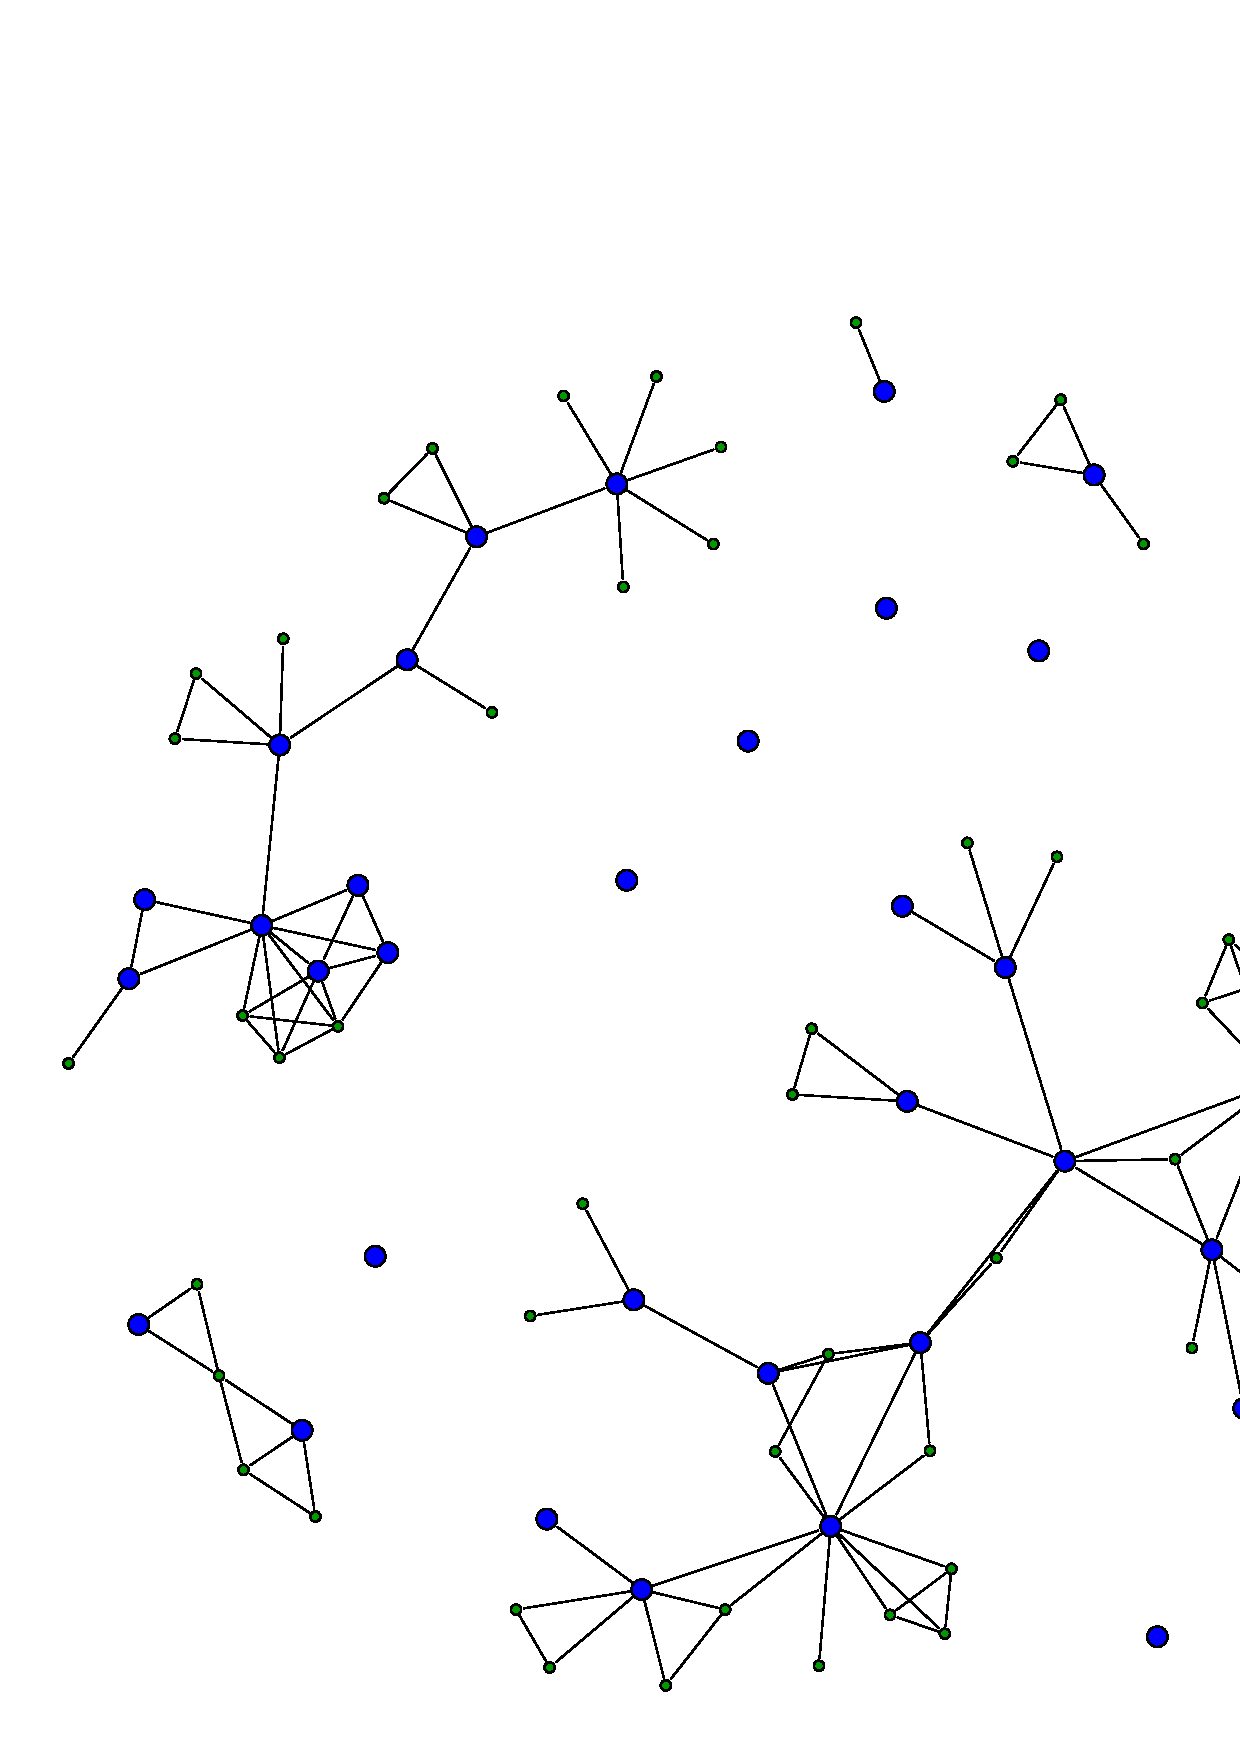
\includegraphics[width=.40\textwidth]{graph} 
  \caption{Descri��o da figura mostrada.}
  \label{fig:humanbeta} 
\end{figure}

%% ------------------------------------------------------------------------- %%
\subsection{Amino�cidos}\index{�cido!amino|(}
\label{sec:amino_acidos}

Veja na Tabela \ref{tab:amino_acidos}...  texto texto texto texto texto texto
texto texto texto texto texto texto texto texto texto texto texto texto texto
texto texto texto texto texto texto texto texto texto texto texto texto texto
texto texto texto texto texto texto texto texto texto texto texto texto texto
texto texto texto texto texto texto texto texto texto texto texto.

\begin{table}[!t]
\begin{center}
    \begin{tabular}{c|c|l}
	 \hline
	 C�digo & Abreviatura & Nome completo \\ \hline
     \texttt{A} & Ala & Alanina \\
     \texttt{C} & Cys & Ciste�na \\
     ...        & ... & ... \\
     \texttt{W} & Trp & Tiptofano \\
     \texttt{Y} & Tyr & Tirosina \\ \hline
    \end{tabular}
  \caption{C�digos, abreviaturas e nomes dos amino�cidos.}
  \label{tab:amino_acidos}
\end{center}
\end{table}
\index{�cido!amino|)}

Texto texto texto texto texto texto texto texto texto texto texto texto texto
texto texto texto texto texto texto texto texto texto texto texto texto texto
texto texto texto texto texto texto texto texto texto texto texto texto texto
texto texto texto texto texto texto texto texto texto texto texto texto texto
texto texto texto texto texto texto texto.


%% ------------------------------------------------------------------------- %%
\section{Exemplo de C�digo-Fonte em Java}
\label{sec:exemplo_codigo_fonte}
Texto texto texto texto texto texto texto texto texto texto texto texto texto
texto texto texto texto texto texto texto texto texto texto texto texto texto
texto texto texto texto texto texto texto texto texto texto texto texto texto
texto texto texto texto texto texto texto.

% Foi utilizado o pacote listing para formatar c�digo fonte
% http://ctan.org/tex-archive/macros/latex/contrib/listings/listings.pdf
% Veja no preambulo do arquivo tese-exemplo.tex os par�metros de configura��o.

\begin{lstlisting}[frame=trbl]
    for(i = 0; i < 20; i++)
    {
        // Coment�rio 
        System.out.println("Mensagem...");
    }
\end{lstlisting}


%% ------------------------------------------------------------------------- %%
\section{Algumas Refer�ncias}
\label{sec:algumas_referencias}

� muito recomend�vel a utiliza��o de arquivos \emph{bibtex} para o gerenciamento
de refer�ncias a trabalhos. Nesse sentido existem tr�s plataformas gratuitas
que permitem a busca de refer�ncias acad�micas em formato bib: 
\begin{itemize}
	\item \emph{CiteULike} (patrocinados por Springer): \url{www.citeulike.org}
	\item Cole��o de bibliografia em Ci�ncia da Computa��o: \url{liinwww.ira.uka.de/bibliography}
	\item Google acad�mico (habilitar bibtex nas prefer�ncias): \url{scholar.google.com.br}
\end{itemize}
Lamentavelmente, ainda n�o existe um mecanismo de verifica��o ou valida��o das
informa��es nessas plataformas. Portanto, � fortemente sugerido validar todas
as informa��es de tal forma que as entradas bib estejam corretas.  Tamb�m, tome
muito cuidado na padroniza��o das refer�ncias bibliogr�ficas: ou considere TODOS
os nomes dos autores por extenso, ou TODOS os nomes dos autores abreviados.
Evite misturas inapropriadas.

Exemplos de refer�ncias com a tag:
\begin{itemize}
\item @Book: \citep{JW82}.
{\scriptsize\begin{verbatim}
@Book{JW82,
 author   = {Richard A. Johnson and Dean W. Wichern},
 title    = {Applied Multivariate Statistical Analysis},
 publisher= {Prentice-Hall},
 year     = {1983}
}
\end{verbatim}}

\item @Article: \citep{MenaChalco08}.
{\scriptsize\begin{verbatim}
@Article{MenaChalco08,
 author   = {Jes�s P. Mena-Chalco and Helaine Carrer and Yossi Zana and 
            Roberto M. Cesar-Jr.},
 title    = {Identification of protein coding regions using the modified 
            {G}abor-wavelet transform},
 journal  = {IEEE/ACM Transactions on Computational Biology and Bioinformatics},
 volume   = {5},
 pages    = {198-207},
 year     = {2008},
}
\end{verbatim}}

\item @InProceedings: \citep{alves03:simi}.
{\scriptsize\begin{verbatim}
@InProceedings{alves03:simi,
 author   = {Carlos E. R. Alves and Edson N. C�ceres and Frank Dehne and 
            Siang W. Song},
 title    = {A Parallel Wavefront Algorithm for Efficient Biological 
            Sequence Comparison},
 booktitle= {ICCSA '03: The 2003 International Conference on Computational Science
            and its Applications},
 year     = {2003},
 pages    = {249-258},
 month    = May,
 publisher= {Springer-Verlag}
}
\end{verbatim}}

\item @InCollection: \citep{bobaoglu93:concepts}.
{\scriptsize\begin{verbatim}
@InCollection{bobaoglu93:concepts,
 author   = {Ozalp Babaoglu and Keith Marzullo},
 title    = {Consistent Global States of Distributed Systems: Fundamental Concepts
            and Mechanisms},
 editor   = {Sape Mullender},
 booktitle= {Distributed Systems},
 edition  = {segunda},
 year     = {1993},
 pages    = {55-96}
}
\end{verbatim}}

\item @Conference: \citep{bronevetsky02}.
{\scriptsize\begin{verbatim}
@Conference{bronevetsky02,
 author   = {Greg Bronevetsky and Daniel Marques and Keshav Pingali and 
            Paul Stodghill},
 title    = {Automated application-level checkpointing of {MPI} programs},
 booktitle= {PPoPP '03: Proceedings of the 9th ACM SIGPLAN Symposium on Principles
            and Practice of Parallel Programming},
 year     = {2003},
 pages    = {84-89}
}
\end{verbatim}}

\item @PhdThesis: \citep{garcia01:PhD}.
{\scriptsize\begin{verbatim}
@PhdThesis{garcia01:PhD,
 author   = {Islene C. Garcia},
 title    = {Vis�es Progressivas de Computa��es Distribu�das},
 school   = {Instituto de Computa��o, Universidade de Campinas, Brasil},
 year     = {2001},
 month    = {Dezembro}
}
\end{verbatim}}

\item @MastersThesis: \citep{schmidt03:MSc}.
{\scriptsize\begin{verbatim}
@MastersThesis{schmidt03:MSc,
 author   = {Rodrigo M. Schmidt},
 title    = {Coleta de Lixo para Protocolos de \emph{Checkpointing}},
 school   = {Instituto de Computa��o, Universidade de Campinas, Brasil},
 year     = {2003},
 month    = Oct
}
\end{verbatim}}

\item @Techreport: \citep{alvisi99:analysisCIC}.
{\scriptsize\begin{verbatim}
@Techreport{alvisi99:analysisCIC,
 author   = {Lorenzo Alvisi and Elmootazbellah Elnozahy and Sriram S. Rao and
            Syed A. Husain and Asanka Del Mel},
 title    = {An Analysis of Comunication-Induced Checkpointing},
 institution= {Department of Computer Science, University of Texas at Austin},
 year     = {1999},
 number   = {TR-99-01},
 address  = {Austin, {USA}}
}
\end{verbatim}}

\item @Manual: \citep{CORBA:spec}.
{\scriptsize\begin{verbatim}
@Manual{CORBA:spec,
 title    = {{CORBA v3.0 Specification}},
 author   = {{Object Management Group}},
 month    = Jul,
 year     = {2002},
 note     = {{OMG Document 02-06-33}}
}
\end{verbatim}}

\item @Misc: \citep{gridftp}.
{\scriptsize\begin{verbatim}
@Misc{gridftp,
 author   = {William Allcock},
 title    = {{GridFTP} protocol specification. {Global Grid Forum}
            Recommendation ({GFD}.20)},
 year     = {2003}
}
\end{verbatim}}

\item @Misc: para refer�ncia a artigo online \citep{fowler04:designDead}.
{\scriptsize\begin{verbatim}
@Misc{fowler04:designDead,
 author   = {Martin Fowler},
 title    = {Is Design Dead?},
 year     = {2004},
 month    = May,
 note     = {�ltimo acesso em 30/1/2010},
 howpublished= {\url{http://martinfowler.com/articles/designDead.html}},
}
\end{verbatim}}

\item @Misc: para refer�ncia a p�gina web \citep{FSF:GNU-GPL}.
{\scriptsize\begin{verbatim}
@Misc{FSF:GNU-GPL,
 author   = {Free Software Foundation},
 title    = {GNU general public license},
 year     = {2007},
 note     = {�ltimo acesso em 30/1/2010},
 howpublished= {\url{http://www.gnu.org/copyleft/gpl.html}},
}
\end{verbatim}}

\end{itemize}

         % associado ao arquivo: 'cap-conceitos.tex'
%% ------------------------------------------------------------------------- %%
\chapter{Conclus�es}
\label{cap:conclusoes}

Texto texto texto texto texto texto texto texto texto texto texto texto texto
texto texto texto texto texto texto texto texto texto texto texto texto texto
texto texto texto texto texto texto\footnote{Exemplo de refer�ncia para p�gina
Web: \url{www.vision.ime.usp.br/~jmena/stuff/tese-exemplo}}.

%------------------------------------------------------
\section{Considera��es Finais} 

Texto texto texto texto texto texto texto texto texto texto texto texto texto
texto texto texto texto texto texto texto texto texto texto texto texto texto
texto texto texto texto texto texto. 

%------------------------------------------------------
\section{Sugest�es para Pesquisas Futuras} 

Texto texto texto texto texto texto texto texto texto texto texto texto texto
texto texto texto texto texto texto texto texto texto texto texto texto texto
texto texto texto texto texto texto.

Finalmente, leia o trabalho de \citet{alon09:how} no qual apresenta-se
uma reflex�o sobre a utiliza��o da Lei de Pareto para tentar definir/escolher
problemas para as diferentes fases da vida acad�mica.  A dire��o dos novos
passos para a continuidade da vida acad�mica deveriam ser discutidos com seu
orientador.
        % associado ao arquivo: 'cap-conclusoes.tex'

% ---------------------------------------------------------------------------- %

% cabe�alho para os ap�ndices
\configurapostextual

\chapter{Sequ�ncias}
\label{ape:sequencias}

Texto texto texto texto texto texto texto texto texto texto texto texto texto
texto texto texto texto texto texto texto texto texto texto texto texto texto
texto texto texto texto texto texto.


\singlespacing

\renewcommand{\arraystretch}{0.85}
\captionsetup{margin=1.0cm}  % corre��o nas margens dos captions.
%--------------------------------------------------------------------------------------
\begin{table}
\begin{center}
\begin{small}
\begin{tabular}{|c|c|c|c|c|c|c|c|c|c|c|c|c|} 
\hline
\emph{Limiar} & 
\multicolumn{3}{c|}{MGWT} & 
\multicolumn{3}{c|}{AMI} &  
\multicolumn{3}{c|}{\emph{Spectrum} de Fourier} & 
\multicolumn{3}{c|}{Caracter�sticas espectrais} \\
\cline{2-4} \cline{5-7} \cline{8-10} \cline{11-13} & 
\emph{Sn} & \emph{Sp} & \emph{AC} & 
\emph{Sn} & \emph{Sp} & \emph{AC} & 
\emph{Sn} & \emph{Sp} & \emph{AC} & 
\emph{Sn} & \emph{Sp} & \emph{AC}\\ \hline \hline
 1 & 1.00 & 0.16 & 0.08 & 1.00 & 0.16 & 0.08 & 1.00 & 0.16 & 0.08 & 1.00 & 0.16 & 0.08 \\
 2 & 1.00 & 0.16 & 0.09 & 1.00 & 0.16 & 0.09 & 1.00 & 0.16 & 0.09 & 1.00 & 0.16 & 0.09 \\
 2 & 1.00 & 0.16 & 0.10 & 1.00 & 0.16 & 0.10 & 1.00 & 0.16 & 0.10 & 1.00 & 0.16 & 0.10 \\
 4 & 1.00 & 0.16 & 0.10 & 1.00 & 0.16 & 0.10 & 1.00 & 0.16 & 0.10 & 1.00 & 0.16 & 0.10 \\
 5 & 1.00 & 0.16 & 0.11 & 1.00 & 0.16 & 0.11 & 1.00 & 0.16 & 0.11 & 1.00 & 0.16 & 0.11 \\
 6 & 1.00 & 0.16 & 0.12 & 1.00 & 0.16 & 0.12 & 1.00 & 0.16 & 0.12 & 1.00 & 0.16 & 0.12 \\
 7 & 1.00 & 0.17 & 0.12 & 1.00 & 0.17 & 0.12 & 1.00 & 0.17 & 0.12 & 1.00 & 0.17 & 0.13 \\
 8 & 1.00 & 0.17 & 0.13 & 1.00 & 0.17 & 0.13 & 1.00 & 0.17 & 0.13 & 1.00 & 0.17 & 0.13 \\
 9 & 1.00 & 0.17 & 0.14 & 1.00 & 0.17 & 0.14 & 1.00 & 0.17 & 0.14 & 1.00 & 0.17 & 0.14 \\
10 & 1.00 & 0.17 & 0.15 & 1.00 & 0.17 & 0.15 & 1.00 & 0.17 & 0.15 & 1.00 & 0.17 & 0.15 \\
11 & 1.00 & 0.17 & 0.15 & 1.00 & 0.17 & 0.15 & 1.00 & 0.17 & 0.15 & 1.00 & 0.17 & 0.15 \\
12 & 1.00 & 0.18 & 0.16 & 1.00 & 0.18 & 0.16 & 1.00 & 0.18 & 0.16 & 1.00 & 0.18 & 0.16 \\
13 & 1.00 & 0.18 & 0.17 & 1.00 & 0.18 & 0.17 & 1.00 & 0.18 & 0.17 & 1.00 & 0.18 & 0.17 \\
14 & 1.00 & 0.18 & 0.17 & 1.00 & 0.18 & 0.17 & 1.00 & 0.18 & 0.17 & 1.00 & 0.18 & 0.17 \\
15 & 1.00 & 0.18 & 0.18 & 1.00 & 0.18 & 0.18 & 1.00 & 0.18 & 0.18 & 1.00 & 0.18 & 0.18 \\
16 & 1.00 & 0.18 & 0.19 & 1.00 & 0.18 & 0.19 & 1.00 & 0.18 & 0.19 & 1.00 & 0.18 & 0.19 \\
17 & 1.00 & 0.19 & 0.19 & 1.00 & 0.19 & 0.19 & 1.00 & 0.19 & 0.19 & 1.00 & 0.19 & 0.19 \\
17 & 1.00 & 0.19 & 0.20 & 1.00 & 0.19 & 0.20 & 1.00 & 0.19 & 0.20 & 1.00 & 0.19 & 0.20 \\
19 & 1.00 & 0.19 & 0.21 & 1.00 & 0.19 & 0.21 & 1.00 & 0.19 & 0.21 & 1.00 & 0.19 & 0.21 \\
20 & 1.00 & 0.19 & 0.22 & 1.00 & 0.19 & 0.22 & 1.00 & 0.19 & 0.22 & 1.00 & 0.19 & 0.22 \\ \hline 
\end{tabular}
\caption{Exemplo de tabela.}
\label{tab:tab:F5}
\end{small}
\end{center}
\end{table}

      	% associado ao arquivo: 'ape-conjuntos.tex'

% bibliografia
\backmatter \singlespacing   			% espa�amento simples
\bibliographystyle{bibliografia/plainnat-ime}   % cita��o bibliogr�fica textual (pode-se usar o "alpha-ime")
\bibliography{bibliografia/bibliografia}        % associado ao arquivo: 'bibliografia.bib'

% indice remissivo
% �ndice remissivo
\index{TBP|see{periodicidade regi�o codificante}}
\index{DSP|see{processamento digital de sinais}}
\index{STFT|see{transformada de Fourier de tempo reduzido}}
\index{DFT|see{transformada discreta de Fourier}}
\index{Fourier!transformada|see{transformada de Fourier}}

\printindex   % imprime o �ndice remissivo no documento 


\end{document}
